\section{Nuclei galattici attivi} \label{sec:nuclei-galattici-attivi}
La radiazione che riceviamo dalla galassie è principalmente dovuta alle stelle. Ma ciò non è vero per tutte le galassie, in particolare ce ne sono alcune in cui si è notato un nucleo centrale estremamente brillante la cui radiazione non è dovuta alle stelle. In altri casi si sono notati delle masse di gas uscenti dalla galassia; il caso più eclatante è quello della galassia Hercules A (in figura~\ref{fig:hercules-a}), in cui si può vedere come nella banda del visibile sia una galassia ellittica, ma quando osservata in banda radio vediamo due spettacolari getti di plasma.

\begin{figure}
    \centering
    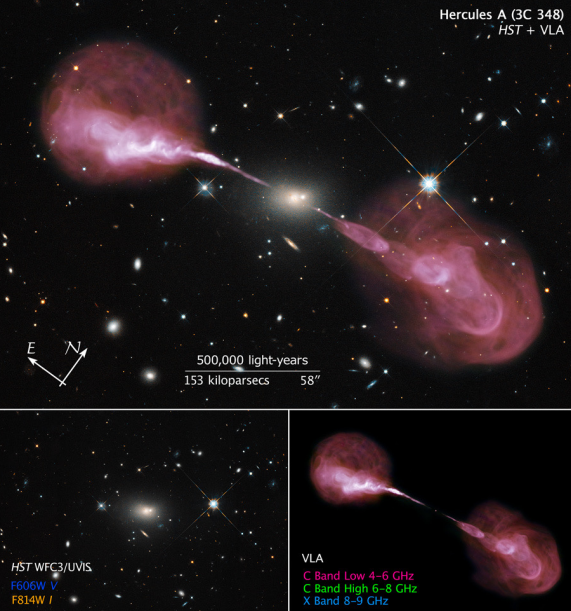
\includegraphics[width = 0.6\textwidth]{immagini/hercules-a.png}
    \caption{Galassia Hercules A (visibile e banda radio). \\ Da notare alcune stelle con la X di luce: sono stelle della NOSTRA galassia.}
    \label{fig:hercules-a}
\end{figure}

La presenza di un nucleo centrale estremamente brillante ma non stellare è tipico dei cosiddetti nuclei galattici attivi (AGN = Active Galactic Nuclei). Un AGN è definito come una regione compatta nel centro di una galassia che emette radiazione che non può essere attribuita a attività stellare ma è in gran parte dovuta a un fenomeno di accrescimento di gas di polvere su un buco nero centrale super massiccio (ossia con massa $> 10^6 \;\si{\solarmass}$). 

\subsection{Proprietà e tassonomia degli AGN}

Le più importanti caratteristiche osservative di una AGN sono:
\begin{itemize}
    \item una luminosità bolometrica molto alta (fino a $L_{bol} \sim 10^{48} \;\si{erg}/\si{s} \sim 3\cdot 10^4 L_{Milky Way}$).
    \item radiazione UV (non stellare), assieme a radiazione infrarossa e visibile.
    \item emissione di raggi X molto intensa.
    \item emissione non termica in un largo range di luminosità.
    \item spettro di emissione permesso con righe spettrali larghe.
    \item spettro di emissione permesso (e proibito) con righe spettrali strette. 
    \item getti relativistici emessi dal nucleo.
    \item variabilità temporale (da minuti ad anni) della continuità delle linee di emissione.
\end{itemize}
Non tutti gli AGN però mostrano queste caratteristiche: è stata sviluppata una tassonomia complicatissima di classi e sottoclassi di AGN sulla base della presenza o assenza di alcune quantità osservate ("AGN zoo").

Una tassonomia semplificata degli AGN può essere fatta in due modi:
\begin{itemize}
    \item Divisione in base allo spettro: indichiamo con AGN di Tipo 1 quelli che hanno linee di emissione sia larghe che strette e con AGN di Tipo 2 quelli che hanno solo linee di emissione strette.
    \item Divisione a seconda dell'emissione in banda radio: 
    \begin{equation*}
        \frac{F_{radio}}{F_{ott}} << 1 \quad \rightarrow \quad \text{RADIO QUIET (Quasars, QSOs, Sayfert galaxies)}
    \end{equation*}
    \begin{equation*}
        \frac{F_{radio}}{F_{ott}} >> 1 \quad \rightarrow \quad \text{RADIO LOUD (Quasars, QSOs, radio galaxies, BL Lac)}
    \end{equation*}
\end{itemize}

\subsection{Tipi di AGN}
\subsubsection{Quasars e QSOs}
Indichiamo con \emph{quasar} (che sta per "quasi-stellar" radio source) un oggetto sorgente di onde radio a distaze cosmologiche, con morfologia puntiforme (quindi simile a una stella) nella banda ottica. 

Indichiamo con \emph{QSOs} (che sta per "quasi-stellar" object) una sorgente di radiazione a distanze cosmologiche che ha morfologia puntiforme (quindi simile a una stella) nella banda ottica, ma con emissione in banda radio nulla o molto debole.

Tutti questi oggetti godono di alcune caratteristiche principali osservate:
\begin{itemize}
    \item sono i più luminosi fra tutti gli AGN ($L_{bol} \sim 10^{45}-10^{48} \;\si{erg}/\si{s}$).
    \item spettro di emissione con larghe linee di emissione permette e strette linee di emissione proibite.
    \item linee spettrali spostate molto verso il rosso.
    \item spesso presentano un colore blu (eccesso di UV) a una temperatura fissa e pari a $T\sim 2.5\cdot 10^4 \;\si{K}$.
    \item 90\% dei quasar sono radio quiet, 10\% sono radio loud.
\end{itemize}

Uno di questi oggetti si chiama 3C 273: è il primo quasar che è stato scoperto e si chiama così perché è il 273esimo oggetto del "Third Cambridge Catalogue of Radio Sources". Di questo oggetto sono stati fatti numerosi studi, in particolare è stata determinata con accuratezza la sua posizione, è stata identificata la sua controparte ottica (ossia la galassia ellittica di cui è il centro) e è stato misurato il suo redshift dalle linee di emissione del visibile. 

\subsubsection{Galassie Seyfert}
Il nome viene dallo scopritore di queste galassie, che ha iniziato a osservarle nel 1943. Sono galassie a disco con alta brillanza superficiale nelle regioni del nucleo (come tutte le AGN) e mostrano righe di emissione molto intense alta luminosità bolometrica ma inferiore di quella dei quasar.
Sono il tipo di AGN più comune nell’universo locale e sono al 95\% radio quiet (emissione in banda radio ma non particolamente forte).

A loro volta sono suddivise in due classi: 
\begin{itemize}
    \item Seyfert 1: forte emissione continua del nucleo non termica, con linee di emissione molto strette ma con spettro molto ampio. Sono inoltre caratterizzate da un'emissione di raggi X intensa e variabile (ore - giorni).
    \item Seyfert 2: Meno luminose delle Seyfert 1, mostrano solo righe di emissione strette (quindi sono AGN di Tipo 2). In più l'emissione di raggi X è molto debole o non presente; il motivo (spiegato più avanti) è che questa radiazione è assorbita da materiale che si interpone tra la Seyfert e noi osservatori. 
\end{itemize}

\subsubsection{Galassie radio}
Come dice il nome sono state classificate in base alla emissione radio; sono galassie con forte emissione radio, la loro luminosità radio confrontabile con i quasar radio loud. Sono caratterizzati dal fatto che la loro galassia è direttamente osservabile (a differenza dei quasar, per i quali è difficile osservare la galassia ospite). Le galassie ospite sono soprattutto galassie ellittiche, ma qualche volta la galassia ospite mostra una morfologia complessa o disturbata, sintomo di una interazione in atto con un'altra galassia. Alcune galassie radio hanno righe di emissione sia larghe che strette, altre hanno solo righe strette 

Anche qui sono presenti due sottoclassi (confronto in figura~\ref{fig:galassie-radio}):
\begin{itemize}
    \item FR I: sono meno lunminose nella banda radio, hanno un continuo ottico e delle righe di emissione più deboli delle FR II. Hanno una discreta varietà di morfologie radio e mostrano dei getti radio molto estesi che partono dal nucleo e si allungano fino a scale dell’ordine dei $\si{Mpc}$; questi getti sono però meno collimati di quelli delle FR II.  
    \item FR II: hanno dei getti radio altamente estesi e collimati e hanno lobi radio che mostrano anche degli hot spots (regioni piccole rispetto al logo dove la brillanza superficiale radio è estremamente elevata). 
\end{itemize}

\begin{figure}
    \centering
    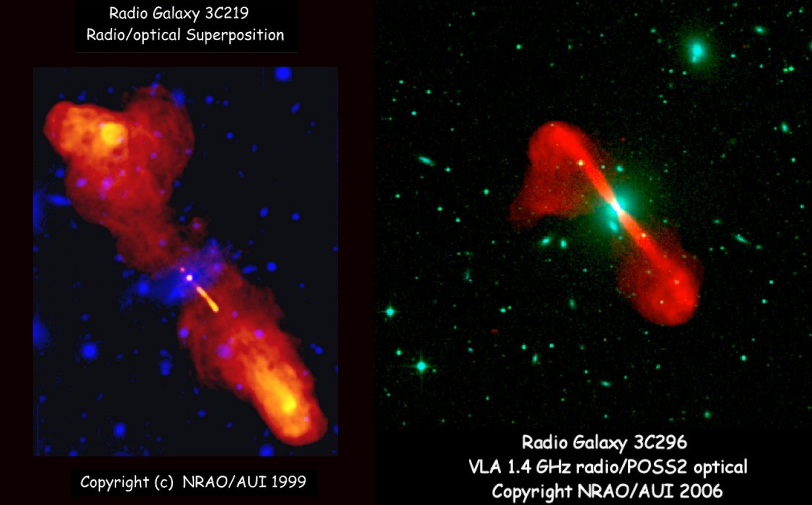
\includegraphics[width = 0.8 \textwidth]{immagini/galassie-radio.png}
    \caption{Confronto fra FR I (destra) e FR II (sinstra): le FR II mostrano raggi più collimati e gli hot spots, assenti invece nelle FR I.}
    \label{fig:galassie-radio}
\end{figure}

\subsubsection{BL Lacertae} 
Il termine BL è usato perchè identifica una classe di stelle variabili e il primo AGN di questo tipo è stato osservato nella costellazione della Lacerta: da lì in poi il nome è questo, solitamente abbreviato in BL Lac. 

Sono contraddistinte da una morfologia star-like (quindi puntiformi), con una variabilità forte e molto rapida (tempi scala brevissimi, fino a circa 10 min); la variabilità dipende dalla lunghezza d’onda (si allunga a lunghezze d’onda più lunga, con i tempi scala che diventano ore ad alte energie, quindi in banda X, e addirittura settimane o mesi nel visibile). Sono molto luminose in banda radio e mostrano un continuo ottico privo di righe (solo di rado si osservano righe di emissione e assorbimento, molto deboli); in più sono molto luminose in gamma. I getti sono orientati a piccoli angoli rispetto alla linea di vista dell’osservatore (circa 20°): ciò significa che non vediamo tutto il getto (90 gradi) ma un getto compattato.

In più sono una sottoclasse delle blazars (sorgenti altamente energetiche, variabili e molto compatte associata a un buco nero supermassiccio situata al centro di una galassia ospitante; sono tra i più violenti fenomeni nell'universo e sono un importante argomento di studio dell'astronomia extragalattica).